%%%%%%%%%%%%%%%%%%%%%%%%%%%%%%%%%%%%%%%%%%%%%%%%%%%%%%%%%%%%%%%%%%%%%%%%%%%%%%%
%                       CARREGA DE LA CLASSE DE DOCUMENT                      %
%                                                                             %
% Les opcions admissibles son:                                                %
%      12pt / 11pt            (cos dels tipus de lletra; no feu servir 10pt)  %
%                                                                             %
% catalan/spanish/english     (llengua principal del treball)                 %
%                                                                             % 
% french/italian/german...    (si necessiteu fer servir alguna altra llengua) %
%                                                                             %
% listoffigures               (El document inclou un Index de figures)        %
% listoftables                (El document inclou un Index de taules)         %
% listofquadres               (El document inclou un Index de quadres)        %
% listofalgorithms            (El document inclou un Index d'algorismes)      %
%                                                                             %
%%%%%%%%%%%%%%%%%%%%%%%%%%%%%%%%%%%%%%%%%%%%%%%%%%%%%%%%%%%%%%%%%%%%%%%%%%%%%%%

\documentclass[11pt,spanish,listoffigures,listoftables]{tfgetsinf}


\usepackage{pgfplotstable} % Para leer y mostrar tablas desde CSV
\usepackage{booktabs}       % Para mejorar el diseño de la tabla
\usepackage{multirow}       % Para fusionar filas
\usepackage{caption}
\usepackage{subcaption}

\usepackage{float}          % Para usar [H] en las figuras
\usepackage{amsmath}        % Para usar \text en modo matemático
%%%%%%%%%%%%%%%%%%%%%%%%%%%%%%%%%%%%%%%%%%%%%%%%%%%%%%%%%%%%%%%%%%%%%%%%%%%%%%%
%                     CODIFICACIO DEL FITXER FONT                             %
%                                                                             %
%    windows fa servir normalment 'ansinew'                                   %
%    amb linux es possible que siga 'latin1' o 'latin9'                       %
%    Pero el mes recomanable es fer servir utf8 (unicode 8)                   %
%                                          (si el vostre editor ho permet)    % 
%%%%%%%%%%%%%%%%%%%%%%%%%%%%%%%%%%%%%%%%%%%%%%%%%%%%%%%%%%%%%%%%%%%%%%%%%%%%%%%

\usepackage[utf8]{inputenc} 
%%%%%%%%%%%%%%%%%%%%%%%%%%%%%%%%%%%%%%%%%%%%%%%%%%%%%%%%%%%%%%%%%%%%%
% Para conseguir que la tabla de contenido no salga en rojo
%%%%%%%%%%%%%%%%%%%%%%%%%%%%%%%%%%%%%%%%%%%%%%%%%%%%%%%%%%%%%%%%%%%%%

\hypersetup{ colorlinks=true, linkcolor=black, urlcolor=cyan, }



%%%%%%%%%%%%%%%%%%%%%%%%%%%%%%%%%%%%%%%%%%%%%%%%%%%%%%%%%%%%%%%%%%%%%%%%%%%%%%%
%                        ALTRES PAQUETS I DEFINICIONS                         %
%                                                                             %
% Carregueu aci els paquets que necessiteu i declareu les comandes i entorns  %
%                                          (aquesta seccio pot ser buida)     %
%%%%%%%%%%%%%%%%%%%%%%%%%%%%%%%%%%%%%%%%%%%%%%%%%%%%%%%%%%%%%%%%%%%%%%%%%%%%%%%



%%%%%%%%%%%%%%%%%%%%%%%%%%%%%%%%%%%%%%%%%%%%%%%%%%%%%%%%%%%%%%%%%%%%%%%%%%%%%%%
%                        DADES DEL TREBALL                                    %
%                                                                             %
% titol, alumne, tutor i curs academic                                        %
%%%%%%%%%%%%%%%%%%%%%%%%%%%%%%%%%%%%%%%%%%%%%%%%%%%%%%%%%%%%%%%%%%%%%%%%%%%%%%%

\title{Detección de defectos en objetos en movimiento mediante Redes Neuronales Convolucionales con optimizaciones específicas para hardware NVIDIA}
\author{Haro Armero, Abel}
\tutor{Flich Cardo, José \\
López Rodríguez, Pedro Juan}
\curs{2024-2025}

%%%%%%%%%%%%%%%%%%%%%%%%%%%%%%%%%%%%%%%%%%%%%%%%%%%%%%%%%%%%%%%%%%%%%%%%%%%%%%%
%                     PARAULES CLAU/PALABRAS CLAVE/KEY WORDS                  %
%                                                                             %
% Independentment de la llengua del treball, s'hi han d'incloure              %
% les paraules clau i el resum en els tres idiomes                            %
%%%%%%%%%%%%%%%%%%%%%%%%%%%%%%%%%%%%%%%%%%%%%%%%%%%%%%%%%%%%%%%%%%%%%%%%%%%%%%%

\keywords{????, ?????????, ????, ?????????????????} % Paraules clau 
         {?????, ???, ???????????????}              % Palabras clave
         {?????, ????? ?????, ?????????????}        % Key words

%%%%%%%%%%%%%%%%%%%%%%%%%%%%%%%%%%%%%%%%%%%%%%%%%%%%%%%%%%%%%%%%%%%%%%%%%%%%%%%
%                              INICI DEL DOCUMENT                             %
%%%%%%%%%%%%%%%%%%%%%%%%%%%%%%%%%%%%%%%%%%%%%%%%%%%%%%%%%%%%%%%%%%%%%%%%%%%%%%%

\begin{document}

%%%%%%%%%%%%%%%%%%%%%%%%%%%%%%%%%%%%%%%%%%%%%%%%%%%%%%%%%%%%%%%%%%%%%%%%%%%%%%%
%              RESUMS DEL TFG EN VALENCIA, CASTELLA I ANGLES                  %
%%%%%%%%%%%%%%%%%%%%%%%%%%%%%%%%%%%%%%%%%%%%%%%%%%%%%%%%%%%%%%%%%%%%%%%%%%%%%%%

\begin{abstract}
????
\end{abstract}
\begin{abstract}[spanish]
????
\end{abstract}
\begin{abstract}[english]
????
\end{abstract}

%%%%%%%%%%%%%%%%%%%%%%%%%%%%%%%%%%%%%%%%%%%%%%%%%%%%%%%%%%%%%%%%%%%%%%%%%%%%%%%
%                              CONTINGUT DEL TREBALL                          %
%%%%%%%%%%%%%%%%%%%%%%%%%%%%%%%%%%%%%%%%%%%%%%%%%%%%%%%%%%%%%%%%%%%%%%%%%%%%%%%

\mainmatter

%%%%%%%%%%%%%%%%%%%%%%%%%%%%%%%%%%%%%%%%%%%%%%%%%%%%%%%%%%%%%%%%%%%%%%%%%%%%%%%
%                                  INTRODUCCIO                                %
%%%%%%%%%%%%%%%%%%%%%%%%%%%%%%%%%%%%%%%%%%%%%%%%%%%%%%%%%%%%%%%%%%%%%%%%%%%%%%%

\chapter{Introducci\'on}
Durante los últimos años, la inteligencia artificial ha experimentado un crecimiento en popularidad sin precedentes, transformando nuestra capacidad tecnológica con herramientas revolucionarias. Este avance ha sido impulsado por la disponibilidad de grandes volúmenes de datos y el desarrollo de algoritmos avanzados, que han permitido a las máquinas aprender y adaptarse a situaciones complejas. Algunos campos destacados de aplicación incluyen el procesamiento del lenguaje natural, la visión por computador y la robótica. En particular, la visión por computador ha visto un auge significativo, con aplicaciones en áreas como la seguridad, la medicina y la automoción. Este creciente interés se refleja en la evolución del interés público en inteligencia artificial, como muestra la Figura~\ref{fig:interes_en_inteligencia_artificial}, basada en datos de Google Trends \cite{googletrends2025}.



\begin{figure}[H]
   \centering
   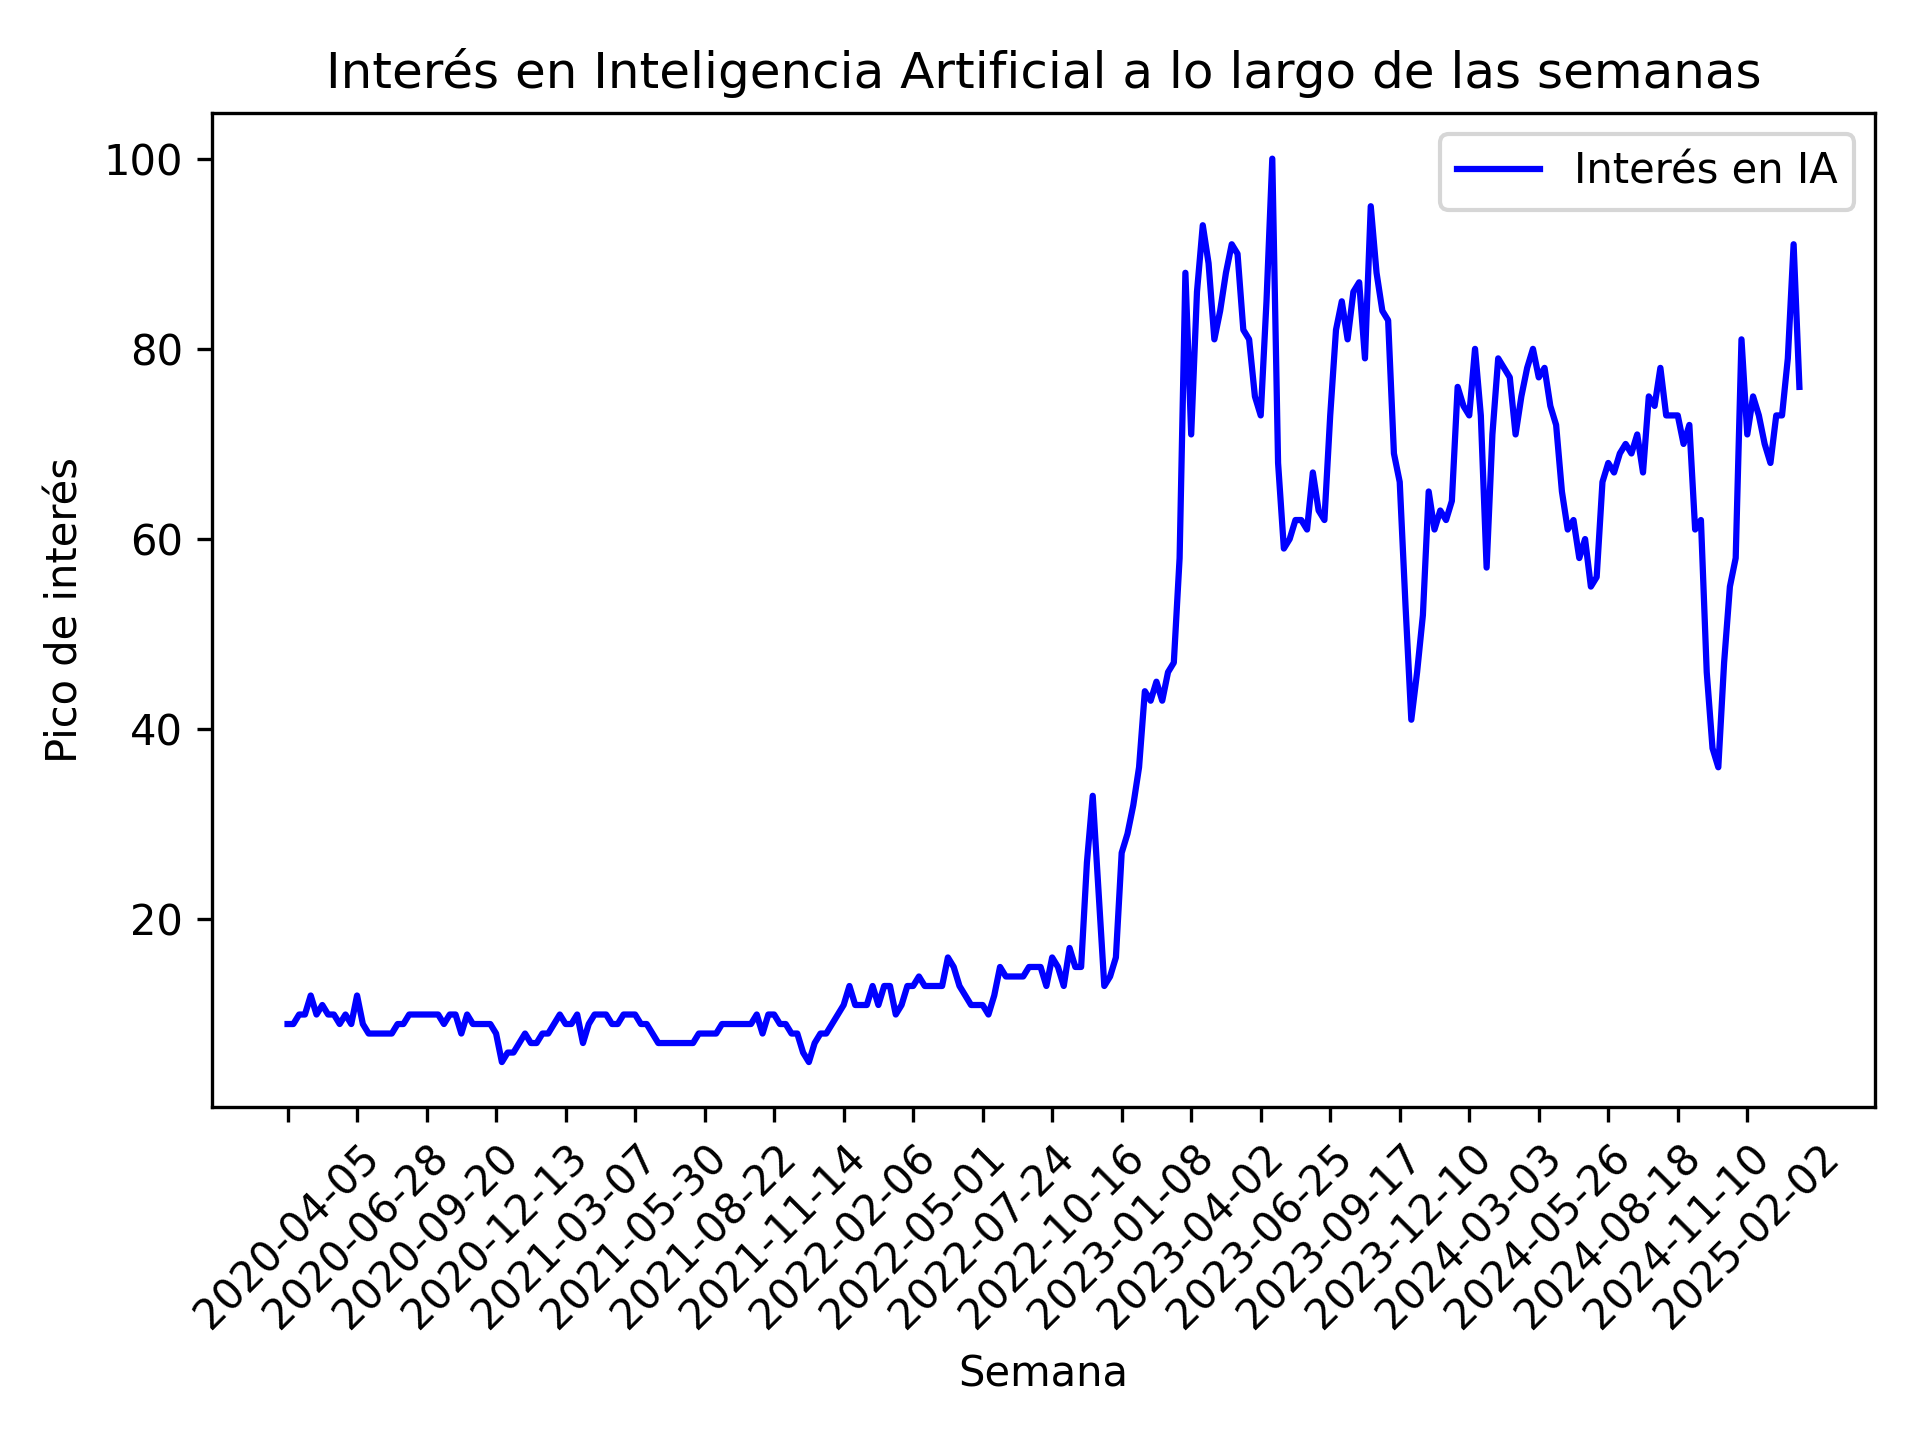
\includegraphics[width=0.7\textwidth]{excels/introduccion/interes_en_ia.png}
   \caption{Evolución del interés público en inteligencia artificial según datos de Google Trends (2020-2025)}
\label{fig:interes_en_inteligencia_artificial}
\end{figure}

Este progreso ha sido posible gracias a los avances en redes neuronales convolucionales, que han revolucionado la capacidad de los sistemas para detectar y clasificar objetos en imágenes y vídeos con una gran precisión y velocidad.

Estos algoritmos de visión artificial requieren una potencia computacional significativa tanto para su entrenamiento como para su ejecución. Las CPUs (Unidades Centrales de Procesamiento) tradicionales resultan insuficientes para estas tareas, por lo que la industria ha desarrollado arquitecturas específicas como las GPUs (Unidades de Procesamiento Gráfico), TPUs (Unidades de Procesamiento Tensorial) y DLAs (Aceleradores de Aprendizaje Profundo). Estos componentes están optimizados para ejecutar operaciones de entrenamiento e inferencia de manera eficiente, permitiendo implementar sistemas de visión artificial capaces de procesar información visual en tiempo real. Sin embargo, estos aceleradores suelen presentar un consumo energético elevado, lo que plantea importantes retos de eficiencia y sostenibilidad.


\begin{figure}[H]
   \centering
   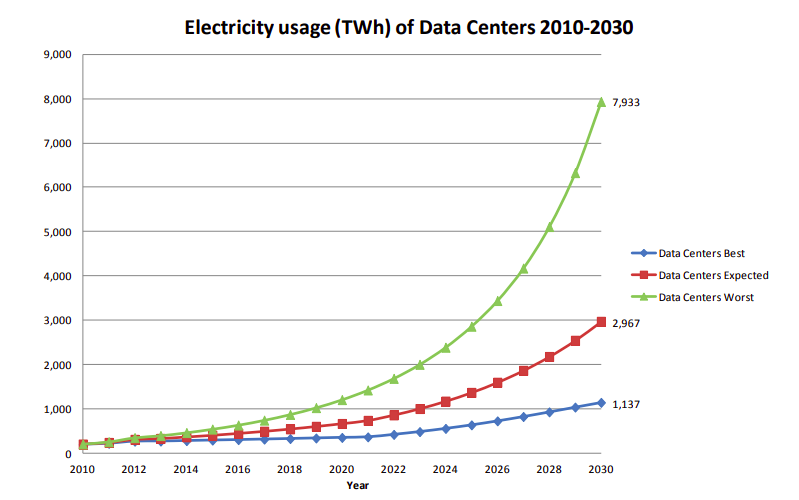
\includegraphics[width=0.7\textwidth]{images/introduccion/consumo_electrico_datacenters.png}
   \caption{Proyección del consumo eléctrico de los centros de datos en el mundo}
\label{fig:consumo_electrico_datacenters}
\end{figure}

Como se observa en la Figura~\ref{fig:consumo_electrico_datacenters}, el consumo eléctrico de los centros de datos en el mundo ha ido aumentando de forma exponencial, lo que plantea un desafío significativo para la sostenibilidad del crecimiento tecnológico \cite{challe6010117}. En el peor escenario, esta tendencia podría llevar a un incremento insostenible en la huella de carbono del sector tecnológico, mientras que en el mejor de los casos, la adopción de tecnologías eficientes podría moderar este crecimiento. Este aumento del consumo energético no solo afecta a los centros de datos, sino también a los dispositivos embebidos y móviles, donde la eficiencia energética es crucial para prolongar la vida útil de las baterías y reducir el impacto ambiental.

Para enfrentar estos desafíos, se han desarrollado diversas técnicas de optimización y compresión que reducen el tamaño y la complejidad de los modelos neuronales manteniendo su rendimiento. Paralelamente, han surgido arquitecturas hardware específicamente diseñadas para la inferencia de modelos de aprendizaje profundo en entornos con restricciones energéticas. En este contexto, los dispositivos de la serie Jetson de NVIDIA destacan por ofrecer un equilibrio entre alto rendimiento en tareas de inteligencia artificial y un consumo energético contenido, ideal para aplicaciones embebidas de visión artificial.

La combinación de redes neuronales convolucionales y aceleradores hardware ha permitido la creación de sistemas de visión artificial que pueden detectar y clasificar objetos en movimiento, lo que es esencial en aplicaciones como la vigilancia, la conducción autónoma y la robótica.

\section{Motivaci\'on}

Los humamos somos capaces de ver y entender el mundo que nos rodea. Dada una imagen, podemos identificar objetos, reconocer patrones y tomar decisiones basadas en la información visual. Sin embargo, esta capacidad no es innata en las máquinas. La visión por computador es la ciencia que busca dotar a las máquinas de la capacidad de interpretar y comprender imágenes y vídeos, emulando la forma en que los humanos percibimos el entorno. 

Como se mencionó anteriormente, la inteligencia artificial ha revolucionado la forma en que interactuamos con la tecnología. Se ha convertido en una herramienta esencial para aplicar soluciones innovadoras en una amplia gama de campos. En particular, la visión por computador ha demostrado ser un área de gran potencial. También la existencia de dispositivos de bajo consumo, como los de la serie Jetson de NVIDIA, ha permitido llevar la inteligencia artificial a entornos de edge computing (cómputo en el borde), donde se acerca el procesamiento de datos a la fuente de información. Esto reduce la latencia y el consumo energético. Con todo esto, se abre un abanico de posibilidades para la implementación de sistemas de visión artificial en aplicaciones industriales.

Centradánose en el ámbito industrial, la detección y clasificación de objetos en movimiento es crucial para optimizar procesos, mejorar la seguridad y aumentar la eficiencia. En la mayoría de entornos productivos, la detección de defectos se realiza de forma manual, lo que puede ser ineficiente y propenso a errores. La automatización de este proceso mediante sistemas de visión artificial puede reducir costos, aumentar la precisión y mejorar la calidad del producto final.


La motivación de este trabajo radica en la necesidad de desarrollar un sistema de visión artificial capaz de detectar y clasificar objetos en movimiento en un entorno industrial, específicamente en una cinta transportadora.


\section{Objetivos}

El objetivo principal de este trabajo es desarrollar un sistema de visión artificial capaz de detectar y clasificar objetos en movimiento en una cinta transportadora utilizando redes neuronales convolucionales y aceleradores hardware de bajo consumo. Para lograr este objetivo, se plantean los siguientes objetivos específicos:

\begin{itemize}
   \item Realizar un estudio del estado del arte en redes neuronales convolucionales, aceleradores hardware de bajo consumo y técnicas avanzadas de optimización para visión artificial.
   \item Desarrollar un conjunto de datos para el entrenamiento y evaluación del sistema, mediante la captura y etiquetado de imágenes de objetos en movimiento.
   \item Diseñar, entrenar y validar un modelo de red neuronal convolucional optimizado para la detección y clasificación en tiempo real de defectos en objetos en movimiento.
   \item Implementar un sistema completo de visión artificial que integre el modelo entrenado con los aceleradores hardware NVIDIA, enfocado en maximizar la eficiencia y minimizar la latencia.
   \item Analizar los cuellos de botella del sistema, y aplicar técnicas específicas de optimización para mejorar el rendimiento y la eficiencia energética.
   \item Cuantificar de manera exhaustiva el rendimiento del sistema mediante métricas precisas de exactitud (mAP, precisión, recall), latencia (FPS) y consumo energético (W, J/inferencia).
   \item Realizar un análisis comparativo sistemático entre diferentes configuraciones de hardware, software y parámetros de optimización para identificar la combinación que ofrezca el mejor equilibrio entre precisión, velocidad y eficiencia energética.
\end{itemize}

\section{Estructura de la memoria}

????? ????????????? ????????????? ????????????? ????????????? ????????????? 

%\section{Notes bibliografiques} %%%%% Opcional

%????? ????????????? ????????????? ????????????? ????????????? ?????????????

%%%%%%%%%%%%%%%%%%%%%%%%%%%%%%%%%%%%%%%%%%%%%%%%%%%%%%%%%%%%%%%%%%%%%%%%%%%%%%%
%                         CAPITOLS (tants com calga)                          %
%%%%%%%%%%%%%%%%%%%%%%%%%%%%%%%%%%%%%%%%%%%%%%%%%%%%%%%%%%%%%%%%%%%%%%%%%%%%%%%

\chapter{Estado del arte}

En este capítulo se realizará un estudio del estado del arte en los diferentes componentes que constituyen la base teórica y técnica de este trabajo. Primero, se examinarán las redes neuronales convolucionales, desde sus fundamentos hasta los modelos más recientes en detección de objetos. A continuación, se analizarán los aceleradores hardware de bajo consumo, con especial énfasis en la arquitectura y capacidades de los dispositivos NVIDIA Jetson. Posteriormente, se estudiarán los algoritmos de seguimiento de objetos en tiempo real, fundamentales para aplicaciones con elementos en movimiento. Finalmente, se explorará la técnica de Slicing Aided Hyper Inference (SAHI), una metodología avanzada para mejorar la detección de objetos pequeños o densamente agrupados. Este marco teórico permitirá contextualizar adecuadamente la solución propuesta para la detección de defectos en objetos en movimiento.

\section{Fundamentos y avances en redes neuronales para visión artificial}
En esta sección se realizará un estudio de las redes neuronales hasta las redes neuronales convolucionales, desde sus fundamentos hasta los modelos más recientes en detección de objetos. Se explicarán los conceptos básicos de las redes neuronales y la evolución de las arquitecturas.

\subsection{Fundamentos de la inteligencia artificial}
La \textit{\textbf{Inteligencia Artificial}} es un campo de estudio que busca desarrollar sistemas capaces de realizar tareas que normalmente requieren inteligencia humana, como el reconocimiento de voz, la toma de decisiones y la comprensión del lenguaje natural. Dentro de este campo, existen diversas subdisciplinas, entre las cuales destacan el \textit{\textbf{Machine Learning}} y el \textit{\textbf{Deep Learning}}.

El \textit{\textbf{Machine Learning}} o aprendizaje automático es una rama de la inteligencia artificial que se centra en el desarrollo de algoritmos y modelos que permiten a las máquinas aprender de los datos y realizar predicciones o tomar decisiones sin ser programadas explícitamente. Este enfoque se basa en la idea de que las máquinas pueden identificar patrones y relaciones en grandes conjuntos de datos, lo que les permite generalizar y adaptarse a nuevas situaciones.

El \textit{\textbf{Deep Learning}} o aprendizaje profundo es una rama del aprendizaje automático que utiliza redes neuronales artificiales con múltiples capas para modelar y resolver problemas complejos. Este enfoque permite aprender representaciones jerárquicas de los datos, donde cada capa extrae características cada vez más abstractas. Una de las arquitecturas fundamentales es el \textit{Multilayer Perceptron} (MLP) o perceptrón multicapa, que consiste en una red de neuronas artificiales organizadas en al menos tres capas: una de entrada, una o más capas ocultas y una capa de salida, como se muestra en la Figura~\ref{fig:multilayer_perceptron} \cite{khan2018guide}. En un MLP, cada neurona recibe un conjunto de entradas ponderadas por pesos, aplica una función de activación no lineal a la suma de estas entradas ponderadas, y produce una salida que se transmite a la siguiente capa. La capacidad de aprendizaje de estas redes se basa en el algoritmo de retropropagación (backpropagation), que ajusta iterativamente los pesos para minimizar el error entre las predicciones de la red y los valores reales. Esta estructura permite al Deep Learning abordar tareas complejas en visión por computador, procesamiento del lenguaje natural y otros dominios con un alto grado de precisión.

\begin{figure}[H]
   \centering
   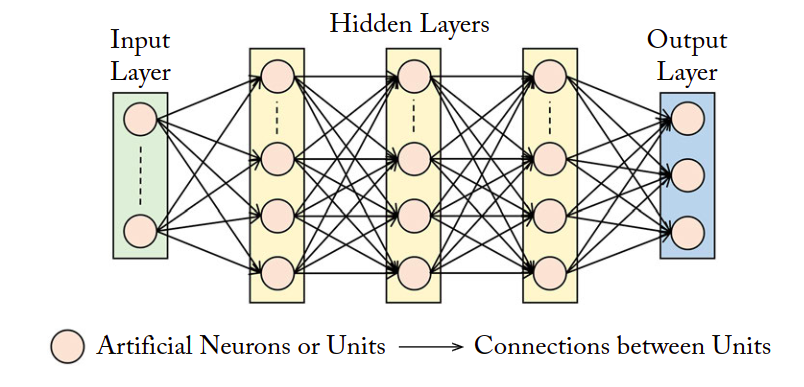
\includegraphics[width=0.6\textwidth]{images/estado_del_arte/multilayer_perceptron.png}
   \caption{Estructura de un perceptrón multicapa (MLP).}
   \label{fig:multilayer_perceptron}
\end{figure}

\subsection{Tareas fundamentales en visión por computador}
En el ámbito del procesamiento de imágenes mediante técnicas de deep learning, existen diversas tareas con diferentes niveles de complejidad:

\begin{enumerate}
    \item \textbf{Clasificación de imágenes}: Es la tarea más básica, donde la red neuronal asigna una etiqueta a toda la imagen. Por ejemplo, determinar si una imagen contiene un perro, gato o coche. El modelo genera un vector de probabilidades para cada clase posible.
    
    \item \textbf{Clasificación con localización}: Además de clasificar el objeto principal, la red también proporciona un cuadro delimitador (bounding box) que indica dónde se encuentra ese objeto en la imagen. Es útil cuando existe un único objeto de interés.
    
   \item \textbf{Detección de objetos}: Extiende la tarea anterior para identificar y localizar múltiples objetos en una imagen. Los algoritmos de detección se dividen principalmente en:
      \begin{itemize}
         \item \textit{Detectores de dos etapas}: Como R-CNN, Fast R-CNN y Faster R-CNN, primero generan propuestas de regiones que podrían contener objetos, y luego clasifican estas regiones. Son más precisos pero computacionalmente más costosos.
         \item \textit{Detectores de una etapa}: Como YOLO (You Only Look Once) y SSD (Single Shot MultiBox Detector), que predicen las cajas delimitadoras y las clases directamente en una sola pasada. Son más rápidos aunque tradicionalmente menos precisos.
      \end{itemize}
      Ambos enfoques proporcionan para cada objeto detectado su clasificación y cuadro delimitador.
    
    \item \textbf{Segmentación}: Es la tarea más compleja, donde la red no solo identifica y localiza objetos, sino que también asigna una etiqueta a cada píxel de la imagen. Esto permite distinguir entre diferentes objetos y sus contornos, facilitando una comprensión más detallada de la escena.
\end{enumerate}

La Figura~\ref{fig:tareas_vision_por_computador} ilustra estas tareas fundamentales en visión por computador. Para este trabajo, nos centraremos en la tarea de detección de objetos, que es esencial para identificar y clasificar varios objetos en movimiento en un vídeo o imagen. 

\begin{figure}[H]
   \centering
   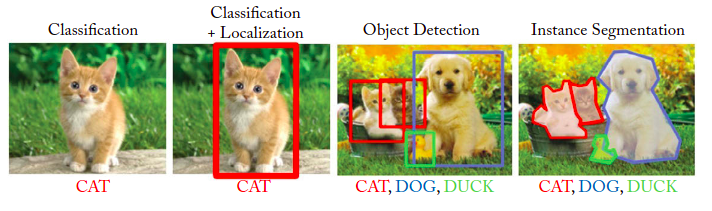
\includegraphics[width=0.8\textwidth]{images/estado_del_arte/diferentes_formas_de_detectar.png}
   \caption{Tareas fundamentales en visión por computador.}
   \label{fig:tareas_vision_por_computador}
\end{figure}

\subsection{Arquitectura y funcionamiento de las CNN}
Las \textit{\textbf{Convolutional Neural Networks}} (CNN) o redes neuronales convolucionales son un tipo específico de red neuronal profunda. Estas redes están diseñadas para procesar imágenes y extraer características relevantes de manera eficiente, lo que las hace especialmente adecuadas para tareas de visión por computador.

\begin{figure}[H]
   \centering
   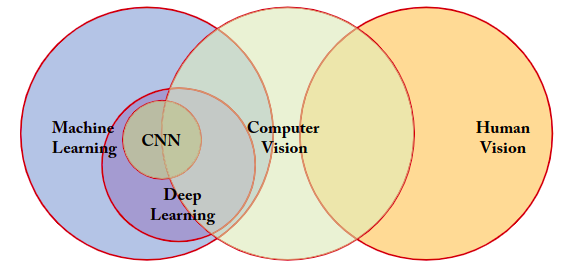
\includegraphics[width=0.6\textwidth]{images/estado_del_arte/diagrama_de_Venn_inteligencia_artificial.png}
   \caption{Relación entre Machine Learning, Deep Learning, CNN, Computer Vision y Human Vision.}
   \label{fig:diagrama_de_Venn_inteligencia_artificial}
\end{figure}

La Figura~\ref{fig:diagrama_de_Venn_inteligencia_artificial} ilustra la relación entre estos conceptos \cite{khan2018guide}. Las CNN son una subcategoría del Deep Learning, que a su vez es una subcategoría del Machine Learning. Además, las CNN están estrechamente relacionadas con la visión por computador, que busca emular la capacidad de los humanos para interpretar imágenes y vídeos.

Las CNN se inspiran en la forma en que los humanos percibimos el mundo visual. Al igual que nuestro sistema visual, que procesa la información de manera jerárquica, las CNN utilizan capas convolucionales para extraer características de bajo nivel (como bordes y texturas) y capas más profundas para identificar patrones y objetos más complejos. Esta jerarquía de características permite a las CNN aprender representaciones ricas y abstractas de los datos visuales.

La operación de convolución es fundamental en las CNN. Esta operación consiste en aplicar un filtro (o kernel) a una imagen para extraer características locales. El filtro se desliza sobre la imagen, multiplicando sus valores por los valores de la imagen en cada posición y sumando los resultados. Este proceso genera un mapa de activación que resalta las características relevantes de la imagen. 

\begin{figure}[H]
   \centering
   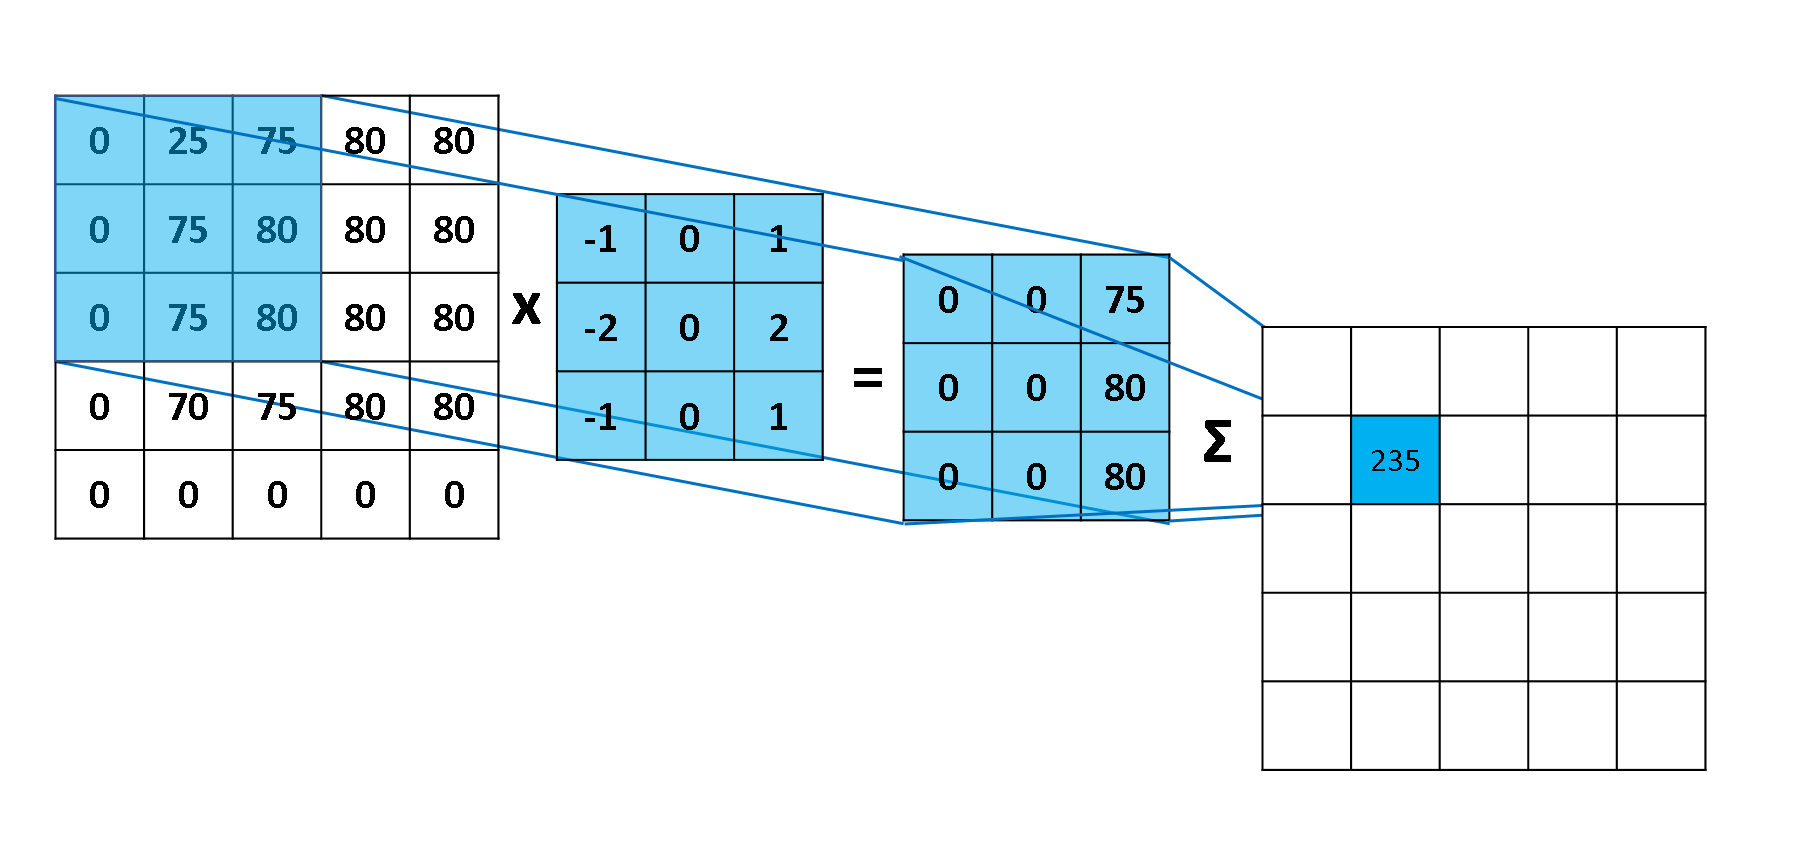
\includegraphics[width=0.6\textwidth]{images/estado_del_arte/operacion_convolucion.png}
   \caption{Operación de convolución en una imagen.}
   \label{fig:operacion_convolucion}
\end{figure}

La Figura~\ref{fig:operacion_convolucion} muestra un ejemplo de la operación de convolución. En este caso, se aplica un filtro de 3x3 a una imagen de entrada, generando un mapa de activación que resalta las características detectadas por el filtro.

\begin{figure}[H]
   \centering
   \begin{subfigure}[b]{0.25\textwidth}
      \centering
      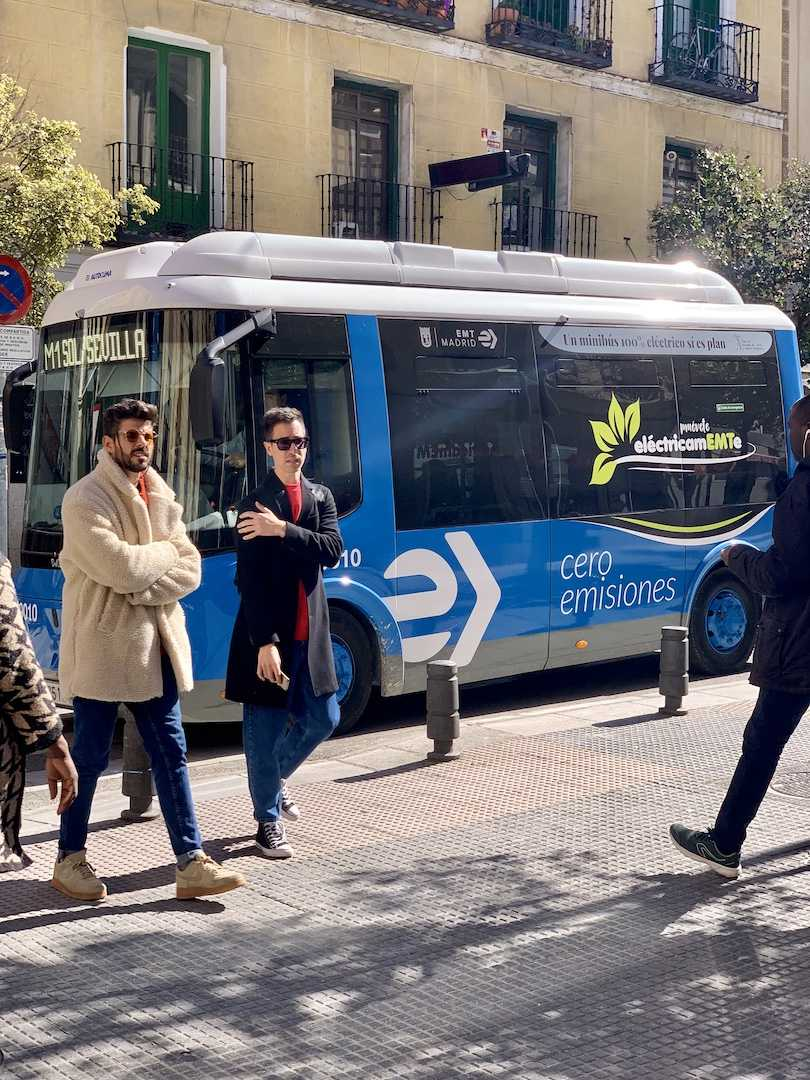
\includegraphics[width=\textwidth]{images/estado_del_arte/bus_original.jpg}
      \caption{Imagen de un autobús.}
      \label{fig:bus_original}
   \end{subfigure}
   \hfill
   \begin{subfigure}[b]{0.7\textwidth}
      \centering
      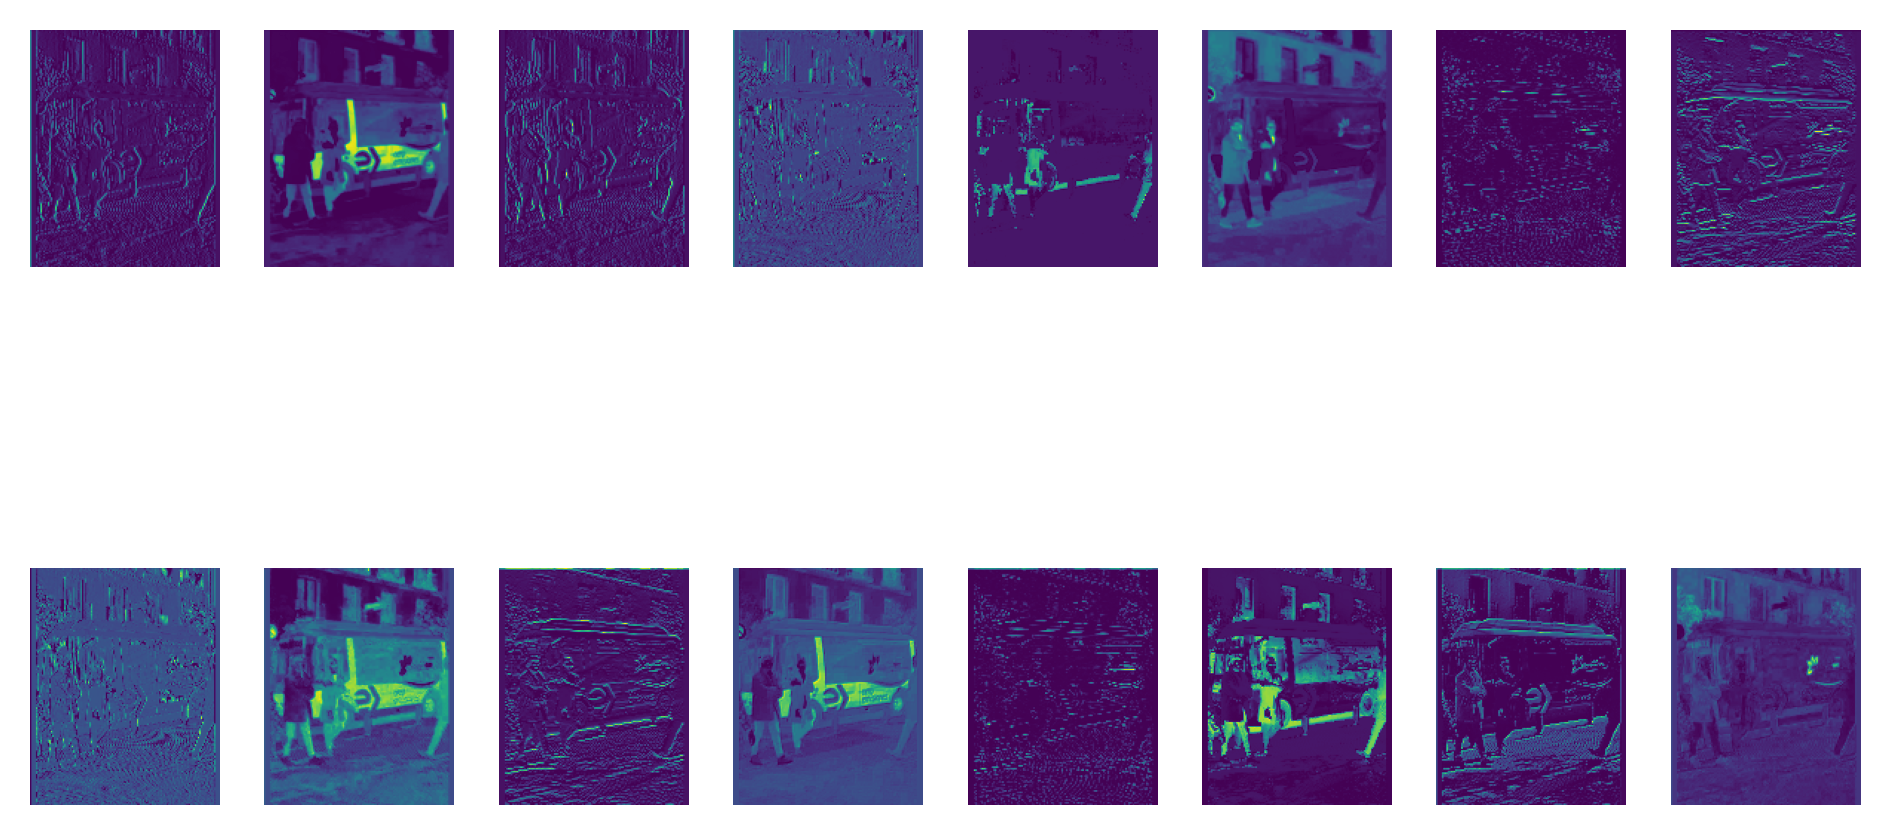
\includegraphics[width=\textwidth]{images/estado_del_arte/bus_primera_capa_convolucion.png}
      \caption{Resultado de la operación de convolución.}
      \label{fig:bus_primera_capa_convolucion}
   \end{subfigure}
   \caption{Proceso de convolución aplicado a una imagen de un autobús.}
   \label{fig:bus_convolucion}
\end{figure}

La Figura~\ref{fig:bus_convolucion} ilustra el proceso de la primera convolución del modelo yolo11n \cite{yolo11_ultralytics}. En la parte izquierda se muestra la imagen original de un autobús, mientras que en la parte derecha se presenta el resultado de aplicar la operación de convolución. En este caso, los 16 filtros de la primera capa convolucional han detectado diferentes características de la imagen, como bordes y texturas. Este proceso se repite en múltiples capas, lo que permite a la red aprender representaciones cada vez más complejas de la imagen.

Además de las capas de convolución, las CNN incluyen capas de \textit{\textbf{pooling}} que permiten reducir la dimensionalidad de las características extraídas, ayudando a prevenir el sobreajuste y a mejorar la eficiencia computacional. El \textit{pooling} consiste en aplicar una operación de reducción (como el máximo o la media) a un conjunto de activaciones, lo que permite resumir la información y mantener las características más relevantes. Este proceso se ilustra en la Figura~\ref{fig:pooling}.

\begin{figure}[H]
   \centering
   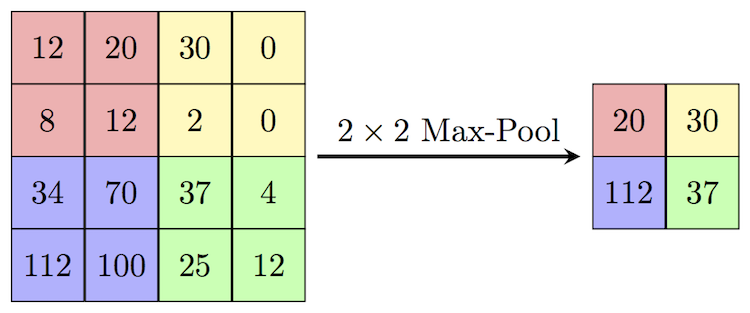
\includegraphics[width=0.6\textwidth]{images/estado_del_arte/max_pooling.png}
   \caption{Operación de max-pooling en una imagen.}
   \label{fig:pooling}
\end{figure}

Por último, las CNN incluyen capas completamente conectadas (\textit{\textbf{fully connected}}) al final de la red, que permiten realizar la clasificación final de los objetos detectados. Estas capas toman las características extraídas por las capas convolucionales y las combinan para generar una salida que representa la probabilidad de que un objeto pertenezca a una clase específica.

En la figura \ref{fig:cnn} se muestra la arquitectura de LeNet-5 \cite{lecun1998gradient}, una de las primeras CNN desarrolladas. Esta red consta de varias capas convolucionales y de pooling, seguidas de capas completamente conectadas. LeNet-5 fue diseñada para la clasificación de dígitos manuscritos y sentó las bases para el desarrollo de arquitecturas más complejas y eficientes en la actualidad.

\begin{figure}[H]
   \centering
   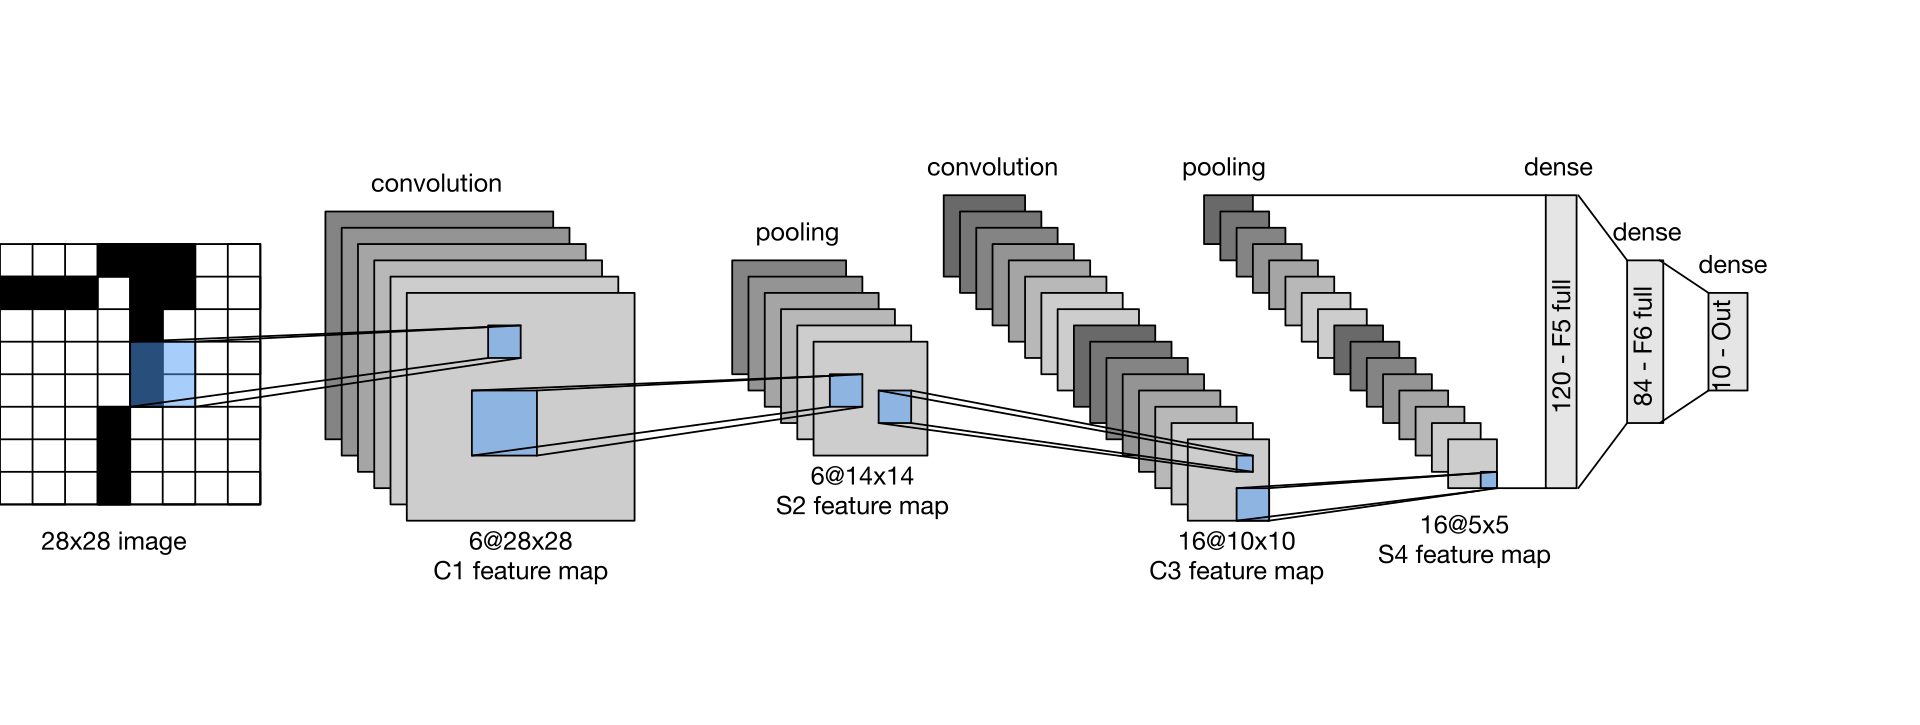
\includegraphics[width=1\textwidth]{images/estado_del_arte/lenet-5.png}
   \caption{Arquitectura de LeNet-5.}
   \label{fig:cnn}
\end{figure}

\subsection{Detectores de dos etapas}
Los detectores de dos etapas, funcionan mediante un proceso secuencial: primero generan propuestas de regiones (region proposals) que podrían contener objetos y posteriormente clasifican estas regiones. Este enfoque favorece la precisión, aunque generalmente a costa de un mayor tiempo de procesamiento.

La primera arquitectura exitosa de detección de objetos basada en deep learning fue R-CNN (Regions with CNN features) \cite{girshick2014richfeaturehierarchiesaccurate}. Este modelo introdujo un enfoque de dos etapas que revolucionó el campo. En su primera fase, R-CNN utiliza un algoritmo de búsqueda selectiva (Selective Search) para generar aproximadamente 2,000 propuestas de regiones que podrían contener objetos. Este algoritmo de búsqueda selectiva divide la imágen en nodos y aristas, e iterativamente agrupa estas regiones en función del color, textura, tamaño y forma hasta que se obtienen las propuestas finales. En la figura \ref{fig:selective_search}\cite{explainningAI} se muestra un ejemplo del resultado del algoritmo de búsqueda selectiva.

\begin{figure}[H]
   \centering
   \begin{subfigure}[b]{0.45\textwidth}
      \centering
      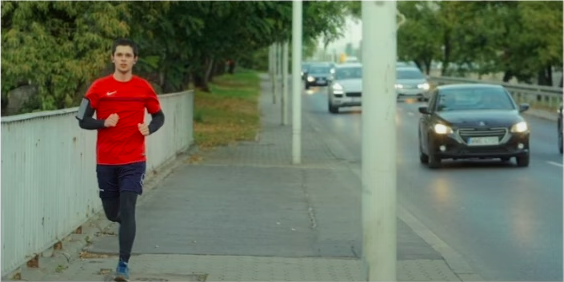
\includegraphics[width=\textwidth]{images/estado_del_arte/selective_search_original.png}
      \caption{Imagen original.}
      \label{fig:selective_search_original}
   \end{subfigure}
   \hfill
   \begin{subfigure}[b]{0.45\textwidth}
      \centering
      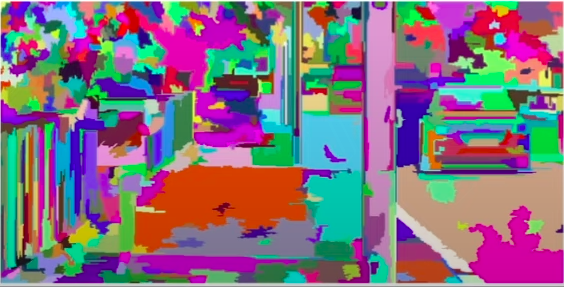
\includegraphics[width=\textwidth]{images/estado_del_arte/selective_search_result.png}
      \caption{Resultado de búsqueda selectiva.}     
      \label{fig:selective_search_result}
   \end{subfigure}
   \caption{Proceso de búsqueda selectiva aplicado a una imagen.}
   \label{fig:selective_search}
\end{figure}

En la segunda fase, cada región propuesta es redimensionada y procesada individualmente por una CNN para extraer características de alto nivel. Estas características alimentan posteriormente a un clasificador SVM (Support Vector Machine) para determinar la categoría del objeto y a un regresor lineal para mejorar la localización del cuadro delimitador. Como se ilustra en la Figura~\ref{fig:r-cnn}, este enfoque fue innovador pero computacionalmente costoso, ya que requiere procesar cada propuesta de región de manera independiente.

\begin{figure}[H]
   \centering
   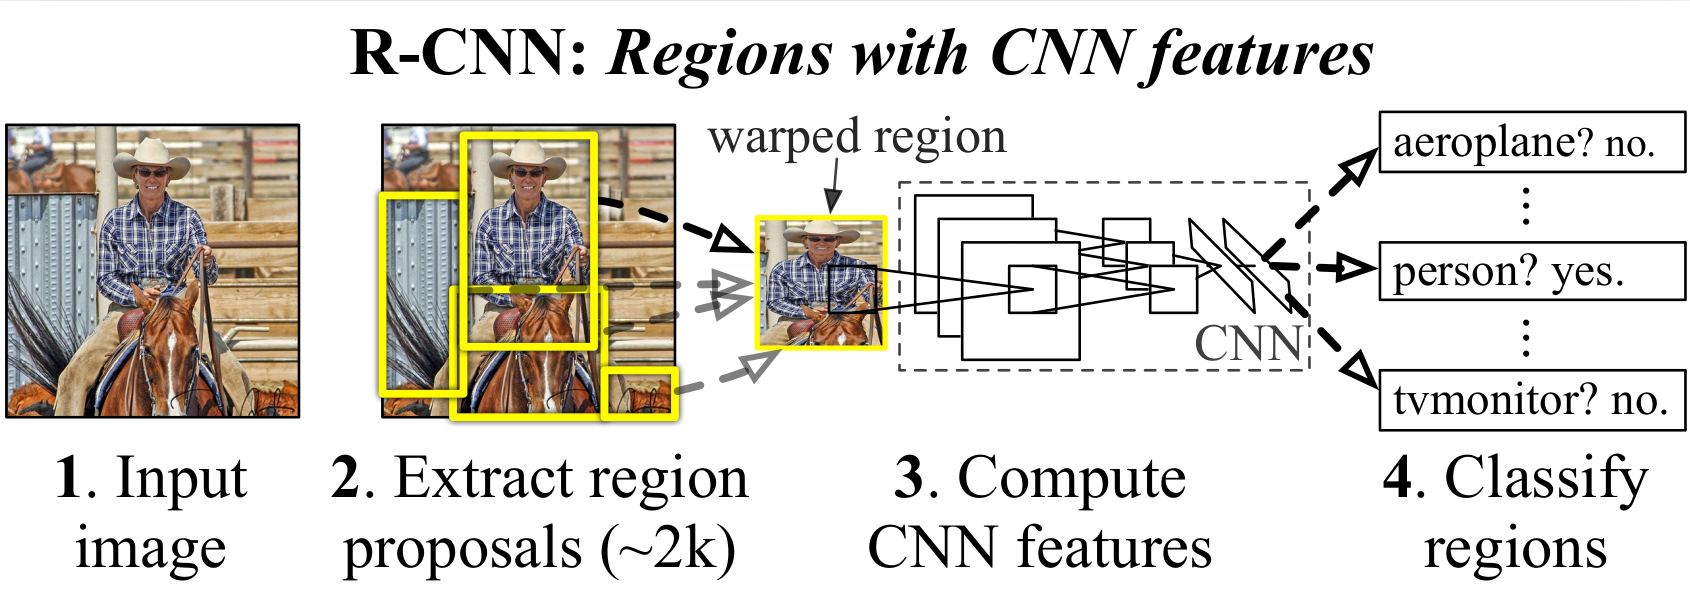
\includegraphics[width=0.6\textwidth]{images/estado_del_arte/R-CNN.png}
   \caption{Arquitectura de R-CNN.}
   \label{fig:r-cnn}
\end{figure}

\subsection{Detectores de una etapa}
%https://www.ultralytics.com/es/glossary/one-stage-object-detectors Explicación de los detectores de 1 etapa por Ultralytics
%https://www.ultralytics.com/glossary/backbone Explicación de la parte de backbone en los detectores de 1 etapa por Ultralytics
%https://www.ultralytics.com/glossary/anchor-free-detectors Explicación de los detectores anchor-free por Ultralytics
%https://sharkyun.medium.com/computer-vision-object-detection-one-stage-vs-two-stage-b05dbff88195 Explicación simple de las diferencias entre los detectores de 2 etapas frente a los de 1 etapa

En contraste con los detectores de dos etapas, los detectores de una etapa (one-stage detectors) adoptan un enfoque más directo y eficiente. Estos detectores realizan la localización y clasificación de objetos simultáneamente en una sola pasada a través de la red, sin necesidad de un paso intermedio de generación de propuestas.

La arquitectura de los detectores de una etapa procesa la imagen completa una única vez, típicamente mediante una red troncal o \textit{backbone} (generalmente una CNN) para la extracción de características. Estas características son posteriormente procesadas por componentes intermedios (\textit{neck}) y alimentadas a una cabeza de detección (\textit{detection head}) que predice simultáneamente las coordenadas de los cuadros delimitadores y las probabilidades de clase. 
Esta arquitectura de una etapa prioriza la velocidad de inferencia, resultando idónea para aplicaciones en tiempo real donde la latencia es un factor crítico, aunque pueda suponer una ligera concesión en la precisión máxima. Modelos representativos de este enfoque incluyen SSD (Single Shot MultiBox Detector)\cite{Liu_2016} y YOLO (You Only Look Once)\cite{redmon2016lookonceunifiedrealtime}. Estos han demostrado un equilibrio eficaz entre rapidez y exactitud, permitiendo la detección en tiempo real incluso en dispositivos con recursos computacionales limitados.

YOLO (You Only Look Once) se destaca como una de las arquitecturas de detección de objetos más populares y efectivas. Concebida específicamente para la detección en tiempo real, YOLO introdujo un enfoque unificado que procesa la imagen completa en una sola pasada, realizando la localización y clasificación de forma simultánea. Esta metodología ha sido fundamental para su adopción en aplicaciones que requieren alta velocidad de procesamiento.

YOLO procesa la imagen completa de una vez. Divide la imagen en una cuadrícula de $S \times S$ celdas. Cada celda es responsable de detectar los objetos cuyo centro se encuentre dentro de ella. Para cada celda, YOLO predice $B$ cuadros delimitadores (bounding boxes) y puntuaciones de confianza para esos cuadros. La puntuación de confianza indica la probabilidad de que haya un objeto en el cuadro y la precisión de la predicción del cuadro. Al mismo tiempo, predice las probabilidades de clase para cada objeto detectado en la celda.

\begin{figure}[H]
   \centering
   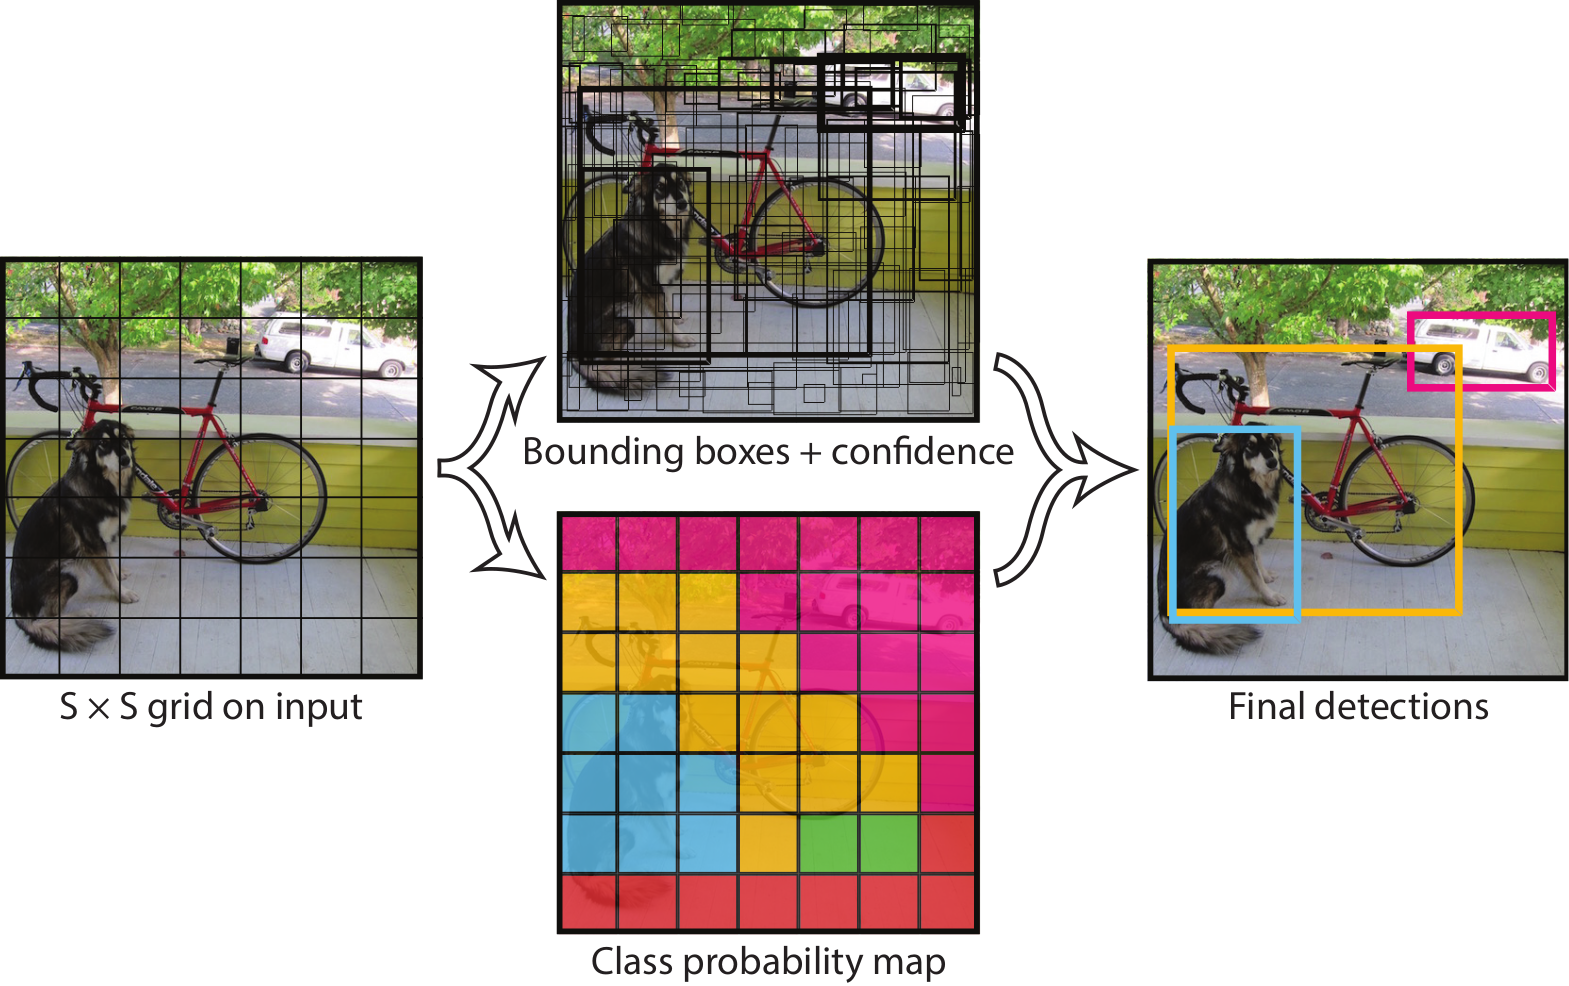
\includegraphics[width=0.8\textwidth]{images/estado_del_arte/yolo_detections_example.png}
   \caption{Ejemplo de detección de objetos utilizando YOLO.}
   \label{fig:yolo_detections_example}
\end{figure}

Como se ilustra en la Figura~\ref{fig:yolo_detections_example}\cite{redmon2016lookonceunifiedrealtime}, YOLO modela la detección como un problema de regresión. Las predicciones del modelo se codifican como un tensor de dimensiones $S \times S \times (B * 5 + C)$, donde el factor $5$ corresponde a las coordenadas $x$, $y$, ancho, alto y la puntuación de confianza para cada cuadro delimitador, mientras que $C$ representa el número de clases posibles. Por ejemplo, si se utilizan $B=2$ cuadros delimitadores y $C=20$ clases, el tensor de salida tendrá dimensiones $S \times S \times (2 * 5 + 20)$. 

Una vez generadas todas las predicciones, YOLO implementa un post-procesamiento mediante supresión de no máximos (NMS) para eliminar detecciones redundantes y conservar únicamente las más precisas. Este enfoque unificado permite que YOLO procese imágenes a velocidades significativamente mayores que los detectores de dos etapas, mientras mantiene una precisión competitiva, lo que lo hace ideal para aplicaciones en tiempo real como las que se abordan en este trabajo.

\begin{figure}[H]
   \centering
   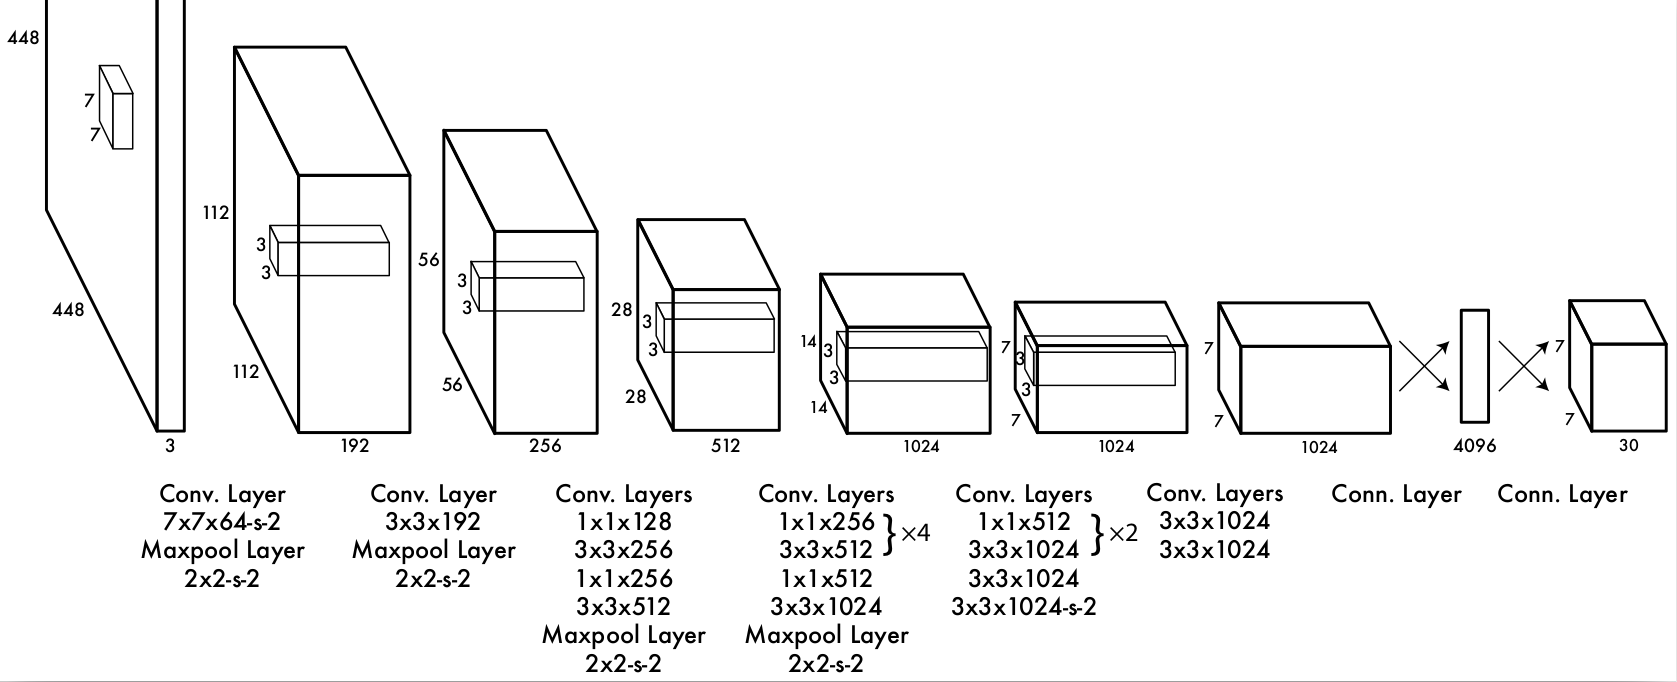
\includegraphics[width=0.8\textwidth]{images/estado_del_arte/yolo_architecture.png}
   \caption{Arquitectura de YOLO}
   \label{fig:yolo_architecture}
\end{figure}

En la Figura~\ref{fig:yolo_architecture} se presenta la arquitectura del modelo primigenio de YOLO \cite{redmon2016lookonceunifiedrealtime}. Esta arquitectura se basa en una red neuronal convolucional que extrae características de la imagen de entrada y las procesa a través de varias capas para generar las predicciones finales. A lo largo de los años, se han desarrollado múltiples versiones y mejoras de YOLO, cada una optimizando aspectos como la precisión, la velocidad y la capacidad de detección de objetos pequeños o densamente agrupados.

En este proyecto, se ha seleccionado YOLO11 \cite{yolo11_ultralytics}, que representa una mejora y optimización sobre las arquitecturas YOLO precedentes. Dicho modelo forma parte de la librería Ultralytics \cite{Jocher_Ultralytics_YOLO_2023}, la cual ofrece una implementación eficaz y sencilla de diversas variantes de YOLO. Las aportaciones de Ultralytics a la comunidad de visión artificial son notables, ya que sus herramientas y recursos agilizan el ciclo de vida (entrenamiento, evaluación, implementación) de los modelos YOLO en múltiples contextos. YOLO11 se ofrece en diversas configuraciones (11n, 11s, 11m, 11l y 11x).
\begin{table}[H]
   \centering
   \resizebox{\textwidth}{!}{%
   \begin{tabular}{l c | cc | c | c}
      \toprule
      Modelo & Tamaño (px) & Latencia CPU ONNX (ms) & Latencia T4 TRT10 (ms) & mAPval (50-95) & Parámetros / FLOPs (M / B) \\
      \midrule
      YOLO11n & 640 & 56.1 ± 0.8 & 1.5 ± 0.0 & 39.5 & 2.6 / 6.5 \\
      YOLO11s & 640 & 90.0 ± 1.2 & 2.5 ± 0.0 & 47.0 & 9.4 / 21.5 \\
      YOLO11m & 640 & 183.2 ± 2.0 & 4.7 ± 0.1 & 51.5 & 20.1 / 68.0 \\
      YOLO11l & 640 & 238.6 ± 1.4 & 6.2 ± 0.1 & 53.4 & 25.3 / 86.9 \\
      YOLO11x & 640 & 462.8 ± 6.7 & 11.3 ± 0.2 & 54.7 & 56.9 / 194.9 \\
      \bottomrule
   \end{tabular}
   }
   \caption{Análisis comparativo de las variantes de YOLO11 considerando precisión, velocidad y complejidad computacional.}
   \label{tab:yolo11_comparison}
\end{table}

La Tabla \ref{tab:yolo11_comparison} presenta un análisis comparativo de las distintas variantes de YOLO11 evaluadas sobre el dataset COCO \cite{lin2015microsoftcococommonobjects}. Los datos revelan una clara correlación: los modelos más grandes ofrecen mayor precisión (mAP) a costa de mayor complejidad computacional y menor velocidad de procesamiento. Esta escalabilidad permite adaptar la implementación según los requisitos específicos de cada aplicación, balanceando efectivamente el rendimiento con las restricciones computacionales del sistema objetivo.

\subsection{Métricas de evaluación}


Para evaluar el rendimiento de los modelos de detección de objetos, se utilizan métricas específicas que permiten cuantificar la precisión y efectividad del sistema. Entre las métricas más comunes se encuentran:

\begin{itemize}
   \item \textbf{Precisión (Precision)}: Mide la proporción de verdaderos positivos (TP) respecto al total de predicciones positivas realizadas por el modelo. Se calcula como:
   \[
   \text{Precision} = \frac{TP}{TP + FP}
   \]
   donde $FP$ representa los falsos positivos. Una alta precisión indica que el modelo realiza pocas predicciones incorrectas.

   \item \textbf{Recall}: Mide la proporción de verdaderos positivos respecto al total de objetos relevantes en la imagen. Se calcula como:
   \[
   \text{Recall} = \frac{TP}{TP + FN}
   \]
   donde $FN$ representa los falsos negativos. Un alto recall indica que el modelo es capaz de detectar la mayoría de los objetos relevantes, aunque pueda incluir algunas predicciones incorrectas.

   \item \textbf{IoU (Intersection over Union)}: Mide la superposición entre el cuadro delimitador predicho y el cuadro delimitador real. Se calcula como:
   \[
   \text{IoU} = \frac{\text{Area de interseccion}}{\text{Area de union}}
   \]

   Una IoU alta indica que el modelo ha localizado correctamente el objeto. Generalmente, se considera que una IoU superior a 0.5 indica una detección correcta.

   \item \textbf{mAP (mean Average Precision)}: Es una métrica que combina precisión y recall, promediando la precisión a diferentes niveles de recall. Se utiliza para evaluar el rendimiento general del modelo en múltiples clases. 
   
   El cálculo del mAP se realiza en varios pasos: primero, para cada clase se calcula la curva PR (Precision-Recall) y se obtiene el Average Precision (AP), que representa el área bajo esta curva. Luego, el mAP se obtiene como la media de todos los AP de las diferentes clases. En detección de objetos, el mAP suele incorporar diferentes umbrales de IoU (Intersection over Union), expresándose como mAP@IoU=0.5 o mAP@IoU=0.5:0.95. Esta métrica es especialmente útil cuando las clases están desequilibradas, ya que da igual importancia a clases minoritarias y mayoritarias. Un valor de mAP cercano a 1 indica un modelo con alta precisión y recall en todas las clases.

   \item \textbf{Latencia}: Mide el tiempo que tarda el modelo en procesar una imagen y generar una predicción se mide en milisegundos (ms) y un valor bajo indica que el modelo es capaz de realizar inferencias rápidamente.
   
   \item \textbf{FPS (Frames Per Second)}: Mide la velocidad de procesamiento del modelo, indicando cuántas imágenes puede procesar por segundo un alto valor de FPS indica que el modelo es capaz de realizar inferencias rápidamente.
   \item \textbf{F1 Score}: Es la media armónica entre precisión y recall, proporcionando un balance entre ambos. Se utiliza para evaluar el rendimiento del modelo en situaciones donde hay un desbalance entre clases. Se calcula como:
   \[
   \text{F1 Score} = 2 \cdot \frac{\text{Precision} \cdot \text{Recall}}{\text{Precision} + \text{Recall}}
   \]

   Un F1 Score alto indica que el modelo tiene un buen equilibrio entre precisión y recall, lo que es especialmente importante en aplicaciones donde tanto la detección correcta como la minimización de falsos positivos son críticas.

\end{itemize}


\section{Aceleradores de procesamiento gráfico}


Un aspecto fundamental para el despliegue eficiente de modelos de inteligencia artificial es el hardware utilizado para su ejecución. A continuación, se analizan los principales aspectos de los aceleradores de procesamiento gráfico y su importancia en aplicaciones de visión artificial.

\subsection{Ventajas de las GPUs para modelos de IA}
A lo largo del desarrollo de la informática, la mejora del hardware ha sido una vía habitual para incrementar el rendimiento de las aplicaciones, permitiendo que los mismos programas funcionen más rápido en procesadores más avanzados. Sin embargo, este enfoque ha ido perdiendo efectividad debido a las limitaciones impuestas por el consumo energético y la disipación térmica, tal como describe la Dennard Scaling. Además, el estancamiento de la ley de Moore ha frenado el avance en el rendimiento de los procesadores convencionales. Como respuesta, han surgido arquitecturas de dominio específico orientadas a maximizar el desempeño en tareas concretas, como las de inteligencia artificial.

Las GPUs (Unidades de Procesamiento Gráfico) representan un claro ejemplo de arquitecturas de dominio específico, diseñadas para maximizar el rendimiento en tareas altamente paralelizables, como las aplicaciones de inteligencia artificial y el procesamiento gráfico. A diferencia de las CPUs tradicionales, que están optimizadas para la ejecución eficiente de una amplia variedad de tareas secuenciales, las GPUs están especializadas en la ejecución simultánea de un gran número de operaciones simples. 

El diseño de las GPUs sigue el paradigma \textit{many-core}, lo que implica la integración de miles de núcleos de procesamiento relativamente simples en un solo chip. Esta arquitectura permite que las GPUs ejecuten múltiples hilos de manera concurrente, lo que resulta especialmente beneficioso para cargas de trabajo que pueden dividirse en tareas independientes, como el procesamiento de grandes volúmenes de datos en redes neuronales profundas.

El modelo de programación de las GPUs está basado en la ejecución masiva de hilos, organizados en bloques y rejillas (\textit{blocks} y \textit{grids}), según la terminología de CUDA, el modelo de programación desarrollado por NVIDIA. Cada hilo ejecuta la misma función, conocida como \textit{kernel}, pero opera sobre diferentes fragmentos de datos. Este enfoque, conocido como SIMD (Single Instruction, Multiple Data), permite aprovechar al máximo el paralelismo inherente a muchas aplicaciones de inteligencia artificial, como el entrenamiento y la inferencia de redes neuronales.

Para programar GPUs, se utilizan lenguajes y APIs especializadas como CUDA y OpenCL, que permiten al desarrollador definir explícitamente cómo se distribuyen los datos y las tareas entre los distintos núcleos de la GPU. El éxito en la programación de GPUs depende en gran medida de la capacidad para identificar y explotar el paralelismo de los algoritmos, así como de una gestión eficiente de la memoria, ya que el acceso a la memoria global de la GPU es mucho más lento que el acceso a la memoria compartida entre hilos de un mismo bloque.

\begin{itemize}
   \item \textbf{Arquitectura de procesamiento paralelo}: Las GPUs contienen miles de núcleos más pequeños diseñados para operaciones simultáneas, mientras que las CPUs tienen menos núcleos pero más potentes.
   
   \item \textbf{Operaciones matriciales eficientes}: Las cargas de trabajo de IA dependen en gran medida de multiplicaciones matriciales, que las GPUs gestionan eficientemente mediante hardware especializado.
   
   \item \textbf{Mayor ancho de banda de memoria}: Las GPUs ofrecen un ancho de banda de memoria significativamente mayor, crucial para procesar grandes conjuntos de datos en redes neuronales.
   
   \item \textbf{Instrucciones especializadas}: Las GPUs modernas incluyen núcleos tensoriales específicamente diseñados para acelerar operaciones de aprendizaje profundo.
   
   \item \textbf{Optimización de rendimiento}: Las GPUs están optimizadas para el procesamiento por lotes en aprendizaje profundo, priorizando el rendimiento sobre la latencia.
\end{itemize}

\subsection{NVIDIA en la aceleración de IA}
NVIDIA ha desempeñado un papel fundamental en el desarrollo de aceleradores para inteligencia artificial:

\begin{itemize}
   \item \textbf{Pionero en GPGPU}: NVIDIA lideró el movimiento de computación de propósito general en GPUs con la introducción de CUDA en 2006.
   
   \item \textbf{Desarrollo del ecosistema}: Creó bibliotecas de software completas (cuDNN, cuBLAS) específicamente para aprendizaje profundo.
   
   \item \textbf{Innovación en hardware}: Desarrolló hardware especializado como los Tensor Cores para operaciones matriciales de IA.
   
   \item \textbf{Estándar de la industria}: Estableció estándares de facto para hardware y software de aceleración de IA.
\end{itemize}

\subsection{Serie Jetson: Dispositivos de IA de bajo consumo}
La serie Jetson de NVIDIA representa una familia de dispositivos específicamente diseñados para implementar IA en el borde:

\begin{itemize}
   \item \textbf{Enfoque en computación edge}: Diseñados para el despliegue de IA en el borde donde existen restricciones de energía.
   
   \item \textbf{Diseño System-on-Chip}: Integra núcleos de CPU ARM, núcleos de GPU NVIDIA y aceleradores especializados.
   
   \item \textbf{Gama de productos}: Abarca desde dispositivos de nivel básico (Jetson Nano) hasta dispositivos de alto rendimiento (Jetson AGX Orin).
   
   \item \textbf{Eficiencia energética}: Ofrece un rendimiento por vatio optimizado para aplicaciones embebidas.
   
   \item \textbf{Plataforma completa}: Proporciona hardware, pila de software y herramientas de desarrollo en un ecosistema unificado.
\end{itemize}

\subsection{TensorRT: Framework de optimización}
TensorRT es un framework desarrollado por NVIDIA para optimizar la inferencia de modelos de aprendizaje profundo:

\begin{itemize}
   \item \textbf{Optimización de inferencia}: Específicamente diseñado para optimizar modelos entrenados para su despliegue.
   
   \item \textbf{Optimización de grafos}: Realiza fusión de capas, calibración de precisión y autoajuste de kernels.
   
   \item \textbf{Soporte de cuantización}: Permite precisión INT8/FP16 para reducir la huella de memoria y aumentar el rendimiento.
   
   \item \textbf{Ajuste específico para plataformas}: Selecciona automáticamente rutas de ejecución óptimas para hardware específico de NVIDIA.
   
   \item \textbf{Capacidades de integración}: Funciona con los principales frameworks como TensorFlow, PyTorch y ONNX.
\end{itemize}



\section{Seguimiento de objetos en tiempo real}
Explicación de como funcionan los algoritmos de multi-object tracking (MOT) en tiempo real, filtro de Kalman hasta BYTETrack.

\section{Slicing Aided Hyper Inference}
Explicación de la técnica de Slicing Aided Hyper Inference, como se utiliza para mejorar la precisión de los modelos de detección de objetos y como se aplica en este trabajo.

\chapter{Análisis del problema}

????? ????????????? ????????????? ????????????? ????????????? ????????????? 

\chapter{Diseño e implementación de la solución}
En este capítulo se explicará la solución propuesta, como se ha diseñado y como se ha implementado.

\section{Descripción del sistema}

Descripción del sistema de visión artificial propuesto, como se ha diseñado y como se ha implementado.

\section{Diseño de las etapas del sistema}

Descripción de las etapas del sistema, como se han diseñado y como se han implementado.

Etapas del sistema:
\begin{itemize}
   \item \textbf{Captura de imágenes:} Descripción de la etapa de captura de imágenes, como se ha diseñado y como se ha implementado.
   \item \textbf{Inferencia:} Descripción de la etapa de inferencia, como se ha diseñado y como se ha implementado.
   \item \textbf{Seguimiento:} Descripción de la etapa de seguimiento, como se ha diseñado y como se ha implementado.
   \item \textbf{Escritura de resultados:} Descripción de la etapa de escritura de resultados, como se ha diseñado y como se ha implementado.
\end{itemize}

\section{Segmentación de las etapas del sistema}

Tipos de segmentación de las etapas del sistema:

\begin{itemize}
   \item \textbf{No segmentada:} Secuencial
   \item \textbf{Segmentación basada en hilos:} Cada etapa del sistema se ejecuta en un hilo diferente.
   \item \textbf{Segmentación basada en procesos:} Cada etapa del sistema se ejecuta en un proceso diferente.
   \item \textbf{Segmentación basada en hardware:} La etapa de inferencia se ejecuta en GPU, DLA0 y DLA1.
   \item \textbf{Segmentación basada en procesos con memoria compartida:} Cada etapa del sistema se ejecuta en un proceso diferente, pero comparten la memoria.
\end{itemize}
    


\chapter{Análisis de la solución}

En este capítulo se analizará la solución propuesta variando los parámetros posibles

\section{Variación de los parámetros}
Explicación de los parámetros que se pueden variar en la solución propuesta y su efecto en el rendimiento del sistema.

------PRUEBA--------


\begin{table}[h]
   \centering
   \resizebox{\textwidth}{!}{ % Ajusta el ancho al tamaño de la página
   \pgfplotstabletypeset[
       col sep=comma, % Definir separador de columnas (por si el CSV usa comas)
       header=true,    % Usar la primera línea como encabezado
       columns={Model, IoU, CPU_Inference, GPU_Inference, DLA_Inference, CPU_Power, GPU_Power, DLA_Power, CPU_Energy, GPU_Energy, DLA_Energy}, % Seleccionar columnas a mostrar
       display columns/0/.style={column name=Model, string type}, % Formato de la columna 'Model'
       display columns/1/.style={column name=IoU}, % Formato de la columna 'IoU'
       display columns/2/.style={column name=CPU\_Inference, column type={|c|}}, % Estilo para columnas de inferencia
       display columns/3/.style={column name=GPU\_Inference, column type={|c|}}, 
       display columns/4/.style={column name=DLA\_Inference, column type={|c|}},
       display columns/5/.style={column name=CPU\_Power, column type={|c|}}, % Estilo para columnas de potencia
       display columns/6/.style={column name=GPU\_Power, column type={|c|}},
       display columns/7/.style={column name=DLA\_Power, column type={|c|}},
       display columns/8/.style={column name=CPU\_Energy, column type={|c|}}, % Estilo para columnas de energía
       display columns/9/.style={column name=GPU\_Energy, column type={|c|}},
       display columns/10/.style={column name=DLA\_Energy, column type={|c|}},
       every head row/.style={before row=\toprule, after row=\midrule}, % Reglas horizontales en el encabezado
       every last row/.style={after row=\bottomrule}, % Reglas horizontales al final
       every column/.style={sci zerofill}, % Opcional, ajusta el formato numérico
       empty cells with={NaN} % Reemplaza celdas vacías o con guiones por NaN
   ]{excels/model_comparasion.csv} % Aquí pones la ruta del archivo CSV
   }
   \caption{Comparación de modelos en términos de inferencia, consumo de energía y potencia.}
   \label{tab:model_comparasion}
\end{table}



------PRUEBA--------



\section{Tipo de segmentación}
En esta sección se analizará el rendimiento de la solución propuesta variando el tipo de segmentación de las etapas del sistema con gráficas y tablas.

\section{Talla del modelo}
En esta sección se analizará el rendimiento de la solución propuesta variando la talla del modelo de detección de objetos con gráficas y tablas.

\section{Precisión del modelo}
En esta sección se analizará el rendimiento de la solución propuesta variando la precisión del modelo de detección de objetos con gráficas y tablas.

\section{Modo de energía y cores de la CPU}
En esta sección se analizará el rendimiento de la solución propuesta variando el modo de energía del dispositivo y el número de cores de la CPU con gráficas y tablas.

\section{Tamaño de la imagen}
En esta sección se analizará el rendimiento de la solución propuesta variando el tamaño de la imagen de entrada del modelo con la técnica de Slicing Aided Hyper Inference (SAHI) con gráficas y tablas.

\chapter{Prueba de concepto}
Aqui se explicará la implementación de la solución propuesta en el entorno de producción con la cinta transportadora.

\section{Construcción del entorno}

\section{Instalación del entorno}






????? ????????????? ????????????? ????????????? ????????????? ?????????????


%%%%%%%%%%%%%%%%%%%%%%%%%%%%%%%%%%%%%%%%%%%%%%%%%%%%%%%%%%%%%%%%%%%%%%%%%%%%%%%
%                                 CONCLUSIONS                                 %
%%%%%%%%%%%%%%%%%%%%%%%%%%%%%%%%%%%%%%%%%%%%%%%%%%%%%%%%%%%%%%%%%%%%%%%%%%%%%%%

\chapter{Conclusiones}

????? ????????????? ????????????? ????????????? ????????????? ????????????? 

%%%%%%%%%%%%%%%%%%%%%%%%%%%%%%%%%%%%%%%%%%%%%%%%%%%%%%%%%%%%%%%%%%%%%%%%%%%%%%%
%                                BIBLIOGRAFIA                                 %
%%%%%%%%%%%%%%%%%%%%%%%%%%%%%%%%%%%%%%%%%%%%%%%%%%%%%%%%%%%%%%%%%%%%%%%%%%%%%%%

\bibliographystyle{plain}      % Estilo de la bibliografía
\bibliography{referencias} % Bibliografia

% \begin{thebibliography}{10}

% %%%%%%%%%%%%%%%%%%%%%%%%%%%%%%%%%%%%%%%%%%%%%%%%%%%%%%%%%%%%%%%%%%%%%%%%%%%%%%%
% % MODEL D'ARTICLE                                                             %
% %%%%%%%%%%%%%%%%%%%%%%%%%%%%%%%%%%%%%%%%%%%%%%%%%%%%%%%%%%%%%%%%%%%%%%%%%%%%%%%
% \bibitem{light}
%    Jennifer~S. Light.
%    \newblock When computers were women.
%    \newblock \textit{Technology and Culture}, 40:3:455--483, juliol, 1999.

% %%%%%%%%%%%%%%%%%%%%%%%%%%%%%%%%%%%%%%%%%%%%%%%%%%%%%%%%%%%%%%%%%%%%%%%%%%%%%%%
% % MODEL DE LLIBRE                                                             %
% %%%%%%%%%%%%%%%%%%%%%%%%%%%%%%%%%%%%%%%%%%%%%%%%%%%%%%%%%%%%%%%%%%%%%%%%%%%%%%%
% \bibitem{ifrah}
%    Georges Ifrah.
%    \newblock \textit{Historia universal de las cifras}.
%    \newblock Espasa Calpe, S.A., Madrid, sisena edició, 2008.

% %%%%%%%%%%%%%%%%%%%%%%%%%%%%%%%%%%%%%%%%%%%%%%%%%%%%%%%%%%%%%%%%%%%%%%%%%%%%%%%
% % MODEL D'URL                                                                 %
% %%%%%%%%%%%%%%%%%%%%%%%%%%%%%%%%%%%%%%%%%%%%%%%%%%%%%%%%%%%%%%%%%%%%%%%%%%%%%%%
% \bibitem{WAR}
% Comunicat de premsa del Departament de la Guerra, 
% emés el 16 de febrer de 1946. 
% \newblock Consultat a 
% \url{http://americanhistory.si.edu/comphist/pr1.pdf}.

% \end{thebibliography}
\cleardoublepage

%%%%%%%%%%%%%%%%%%%%%%%%%%%%%%%%%%%%%%%%%%%%%%%%%%%%%%%%%%%%%%%%%%%%%%%%%%%%%%%
%                           APÈNDIXS  (Si n'hi ha!)                           %
%%%%%%%%%%%%%%%%%%%%%%%%%%%%%%%%%%%%%%%%%%%%%%%%%%%%%%%%%%%%%%%%%%%%%%%%%%%%%%%

\APPENDIX

%%%%%%%%%%%%%%%%%%%%%%%%%%%%%%%%%%%%%%%%%%%%%%%%%%%%%%%%%%%%%%%%%%%%%%%%%%%%%%%
%                         LA CONFIGURACIO DEL SISTEMA                         %
%%%%%%%%%%%%%%%%%%%%%%%%%%%%%%%%%%%%%%%%%%%%%%%%%%%%%%%%%%%%%%%%%%%%%%%%%%%%%%%

\chapter{Configuración del sistema}

????? ????????????? ????????????? ????????????? ????????????? ?????????????

\section{Fase de inicialitzación}

????? ????????????? ????????????? ????????????? ????????????? ?????????????

\section{Identificación de dispositivos}

????? ????????????? ????????????? ????????????? ????????????? ?????????????

%%%%%%%%%%%%%%%%%%%%%%%%%%%%%%%%%%%%%%%%%%%%%%%%%%%%%%%%%%%%%%%%%%%%%%%%%%%%%%%
%                               ALTRES  APÈNDIXS                              %
%%%%%%%%%%%%%%%%%%%%%%%%%%%%%%%%%%%%%%%%%%%%%%%%%%%%%%%%%%%%%%%%%%%%%%%%%%%%%%%


\chapter{??? ???????????? ????}

????? ????????????? ????????????? ????????????? ????????????? ????????????? 



%%%%%%%%%%%%%%%%%%%%%%%%%%%%%%%%%%%%%%%%%%%%%%%%%%%%%%%%%%%%%%%%%%%%%%%%%%%%%%%
%                              FI DEL DOCUMENT                                %
%%%%%%%%%%%%%%%%%%%%%%%%%%%%%%%%%%%%%%%%%%%%%%%%%%%%%%%%%%%%%%%%%%%%%%%%%%%%%%%

\end{document}
